% Created 2020-09-18 Fri 10:31
% Intended LaTeX compiler: pdflatex
\documentclass[11pt]{article}
\usepackage[utf8]{inputenc}
\usepackage[T1]{fontenc}
\usepackage{graphicx}
\usepackage{grffile}
\usepackage{longtable}
\usepackage{wrapfig}
\usepackage{rotating}
\usepackage[normalem]{ulem}
\usepackage{amsmath}
\usepackage{textcomp}
\usepackage{amssymb}
\usepackage{capt-of}
\usepackage{hyperref}
\author{adam}
\date{\today}
\title{}
\hypersetup{
 pdfauthor={adam},
 pdftitle={},
 pdfkeywords={},
 pdfsubject={},
 pdfcreator={Emacs 26.3 (Org mode 9.3.8)}, 
 pdflang={English}}
\begin{document}

\tableofcontents

\section{Overview}
\label{sec:orgdca4efa}

\subsection{Course Structure}
\label{sec:org089afb5}
This course is an introduction to media theory – a subcategory of
philosophy that emerged in the mid 20th century as an attempt to
understand the impact that new technologies were having on the
individual and, in a broader sense, society. 
The general tone used to convey the ideas contained throughout the
notes and lectures will be an informal one, you refers to you the
reader, listener and student. We refers to the teachers, authors and 
students that have been consulted in developing the material for this 
course. Us refers to the group that we happen to find ourselves in at 
any particular moment in time. And I refers to me, the teacher, Adam McCartney.  
This course is intended to introduce undergraduate level music
students to the broader disciplines relevant for professional work in 
the arts and humanities. There are those who would consider it absurd 
that now, in the 21st century, investing in anything but a science
related degree is simply a waste. In the face of such beliefs, it is 
worth pausing briefly to remember a simple point made by John Henry
Newman, that a solid education in the liberal arts equips a student
with tools that will ultimately lead them to become better engineers, 
scientists, doctors, artists, lawyers and etc.   


\subsection{Philosophy of Teaching}
\label{sec:orgd6be684}
\begin{center}
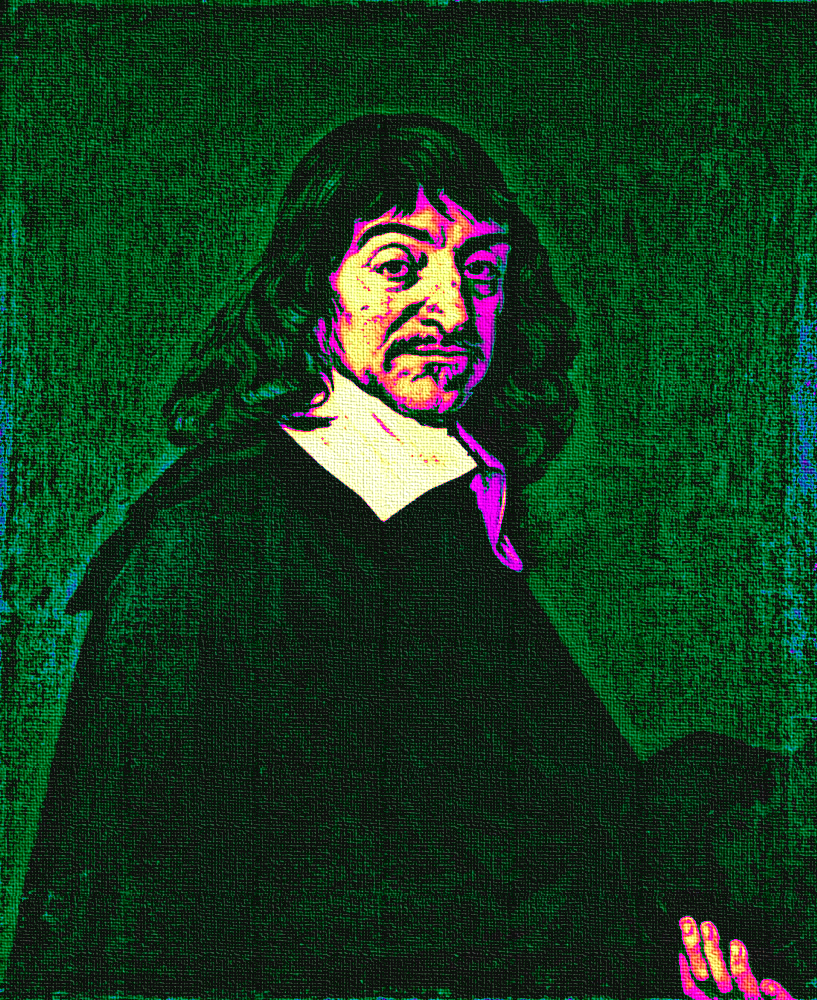
\includegraphics[width=.9\linewidth]{./descartes.png}
\end{center}
The satisfaction that can be gained through learning, teaching and
generally sharing information and can be immense. My more positive 
experiences over the years as a student and teacher have tended to 
come from courses, books, tutorials, videos, discussions that were 
clear enough to allow enable an understanding of the topic from 
first principles – that is to say that the material related to 
the topic was assembled in such a way as to reveal its most
fundamental ideas. Its virtually always beneficial to ask rudimentary 
questions about whatever it is that we are trying to understand, as 
such questions will quickly reveal whether or not the topic under 
discussion has a basis in fact. 
This course also aims to introduce some of the core methods that are
useful anywhere that it becomes necessary to think about something:

\begin{itemize}
\item Discourse
\item Reason
\item Logic
\item Debate
\item Reference
\end{itemize}


\subsubsection{7 Liberal Arts of the medieval university}
\label{sec:org85c0110}
\begin{itemize}
\item Grammar
\item Rhetoric
\item Logic
\item Geometry
\item Arithmetic
\item Music
\item Astronomy
\end{itemize}

\subsection{Where and how to access material}
\label{sec:orgb216062}
The primary source of information for topics presented in this course
can be found in the VMI digital library, which is labelled \emph{Academic
Resources For Students} and will appear as a link on the homepage of
your Moodle eLearning profile. 
Please take the time to do the readings, this will prepare you for the
discussions that will take place during class. Thinking about things
is a practical exercise, it‘s the same as riding a bicycle or learning
to play an instrument. That means that the only way that you are going
to learn how to think is by engaging with the readings and
exercises. Much the same as any activity that is worth learning,
thinking is difficult and takes a lot of patience to get right. 
The texts that were chosen to be part of the course are all written in
an accessible style and are not overtly academic or
technical. Nevertheless, they do contain  ideas and arguments that you
might not get on the first reading.  My two favorite reading
disciplines  from when I was an undergraduate were the practice of
reading for a pre-allocated amount of time and also reading each text
at least three times in preparation for a class. 

\subsection{Portability and how to apply course content}
\label{sec:org103ef98}
Should you try and tell your piano tuner about Ludwig Wittgenstein‘s
ideas on the formation of knowledge? Definitely not! In fact, they
would be more likely to charge you extra fees just to get your piano
tuned if you chose to do so. 
So where exactly can this knowledge be applied? A friend of mine is a
hobby programmer and he recently told me his principle approach to
work. He called it „eat your own dogfood“. Now obviously the idea of
eating any kind of dogfood does not sound particularly appetizing, but
it is worth considering that dogs can also eat cake. The simple idea
here is that whatever type of idea or discipline you develop, it is
better first practiced on yourself before inflicting it upon the rest
of us; when properly cultivated a discipline is a way to nourish,
develop and sustain.




\section{A brief history of society, thought and ideas in the post industrial world}
\label{sec:orgf51378a}

\subsection{The long 19th century (1789 - 1914)}
\label{sec:org6c6702a}
\subsection{The short 20th century (1914 - 1996)}
\label{sec:org99756ba}

\subsection{Walther Benjamin}
\label{sec:org8a09f35}
\subsubsection{The Work of Art in the Age of Mechanical Reproduction}
\label{sec:orgad8d373}

\section{Historical context for media theory}
\label{sec:orga1fcc97}
\subsection{Marshall McCluhan}
\label{sec:orgcf9a0db}
\subsubsection{The Medium is the message}
\label{sec:org7f236f1}
\url{https://web.mit.edu/allanmc/www/mcluhan.mediummessage.pdf}

\section{Hackers and the open source movement}
\label{sec:org0938e33}

\subsection{Eric Raymond}
\label{sec:org42034ff}
\subsubsection{How to become a hacker}
\label{sec:org9e1e646}
\url{http://www.catb.org/esr/faqs/hacker-howto.html}
\subsubsection{The new hacker's dictionary}
\label{sec:orgb52387e}
\url{http://hackersdictionary.com/html/index.html}

\section{Navigating the digital world in the time of soul sucking mega corporations}
\label{sec:orge0776e8}

\subsection{Douglas Rushkoff and Team Human}
\label{sec:org9d0a5af}
\subsubsection{Program or be Programmed}
\label{sec:org7a64a2f}
\url{https://www.youtube.com/watch?v=imV3pPIUy1k\&feature=youtu.be}

\subsubsection{Team Human Podcast}
\label{sec:orgce0b60c}
\url{https://teamhuman.fm}

\section{A brief history of epistemology}
\label{sec:orgf073aa0}
\subsection{A few short points on the formation of knowledge}
\label{sec:org581777b}
\subsubsection{Ancient}
\label{sec:org20cafe1}
\subsubsection{Early Modern}
\label{sec:orgd5bec3d}
\subsubsection{National States Period}
\label{sec:org37ed487}
\subsubsection{Contemporary Perspectives}
\label{sec:orgd95881f}

\section{Adaptation and Adoption}
\label{sec:org8134858}
\subsection{Features of Intagibles}
\label{sec:orge550a1e}
\subsection{Shared Strategies – the automaton blues}
\label{sec:org1482a7e}

\section{Course Work}
\label{sec:orgd390cef}
Semester requirements are to do the readings, and submit two essays,
one short (ca. 1000 words) and one longer (ca. 2500 words). Actually,
the medium that you present these works is flexible - in the past
students have produced podcasts, written essays, made lesson
plans. The important thing is that you work on forming an idea an
presenting it in a coherant way. 

\subsection{Where are the best places to borrow ideas?}
\label{sec:orga8bea41}
\subsection{Can we please make music theory a little less boring?}
\label{sec:org23818ea}
\end{document}
